\documentclass[11pt,leqno]{article}
\usepackage[T1]{fontenc}
\usepackage[polish]{babel}
\usepackage[utf8]{inputenc}
\usepackage{a4wide}
\usepackage{amsmath}
\usepackage{graphicx}

\title{
  \textbf{Pracownia z analizy numerycznej}\\
  \textit{Zadanie 2}
}
\author{Łukasz Hanuszczak}
\date{Wrocław, \today}

\begin{document}
\maketitle



\section{Wstęp}


Ułamkiem łańcuchowym nazywamy ułamek postaci
\[
x =
  a_0 + \frac{1}{\displaystyle
    a_1 + \frac{1}{\displaystyle
      a_2 + \frac{1}{\displaystyle
        a_3 + \dots
      }
    }
  }
\]
gdzie $a_0, a_1, a_2, \dots$ są liczbami całkowitymi nazywanymi współczynnikami ułamka. Ułamek może być skończony bądź nieskończony. W pierwszym przypadku jego wartością jest liczba wymierna, w drugim - niewymierna.

Ułamki łańcuchowe posiadają wiele ciekawych własności, między innymi to że każdej liczbie wymiernej odpowiada dokładnie jeden ułamek łańcuchowy w formie kanonicznej (tj. takiej, że ostatni współczynnik nie jest postaci $\frac{1}{1}$). Aby otrzymać reprezentację danej liczby wymiernej w postaci ułamka łańcuchowego można wykorzystać algorytm Euklidesa, gdzie kolejne iteracje będą zwracać jego współczynniki.

Zadanie polega na obliczaniu wartości uogólnionej formy ułamków łańcuchowych, to jest ułamkamków postaci
\[
x =
  b_0 + \frac{a_1}{\displaystyle
    b_1 + \frac{a_2}{\displaystyle
      b_2 + \frac{a_3}{\displaystyle
        b_3 + \dots
      }
    }
  }
\]
O ile postać ta jest mniej ,,ciekawa'' jeżeli chodzi o własności to ma bardziej praktyczne zastosowanie.

Wprowadza się również pojęcie zbieżnika\footnote{autorskie tłumaczenie angielskiego \emph{convergent}, którego oficjalnego tłumaczenia nigdzie nie mogłem odnaleźć.}, który oznacza ,,obcięty'' fragment ułamka łańcuchowego. Dla powyższego ułamka ciąg zbieżników prezentuje się następująco
\[
  x_0 = b_0,
  x_1 = b_0 + \frac{a_1}{\displaystyle
    b_1
  },
  x_2 = b_0 + \frac{a_1}{\displaystyle
    b_1 + \frac{a_2}{\displaystyle
      b_2
    }
  },
  \dots,
  x_i = b_0 + \frac{a_1}{\displaystyle
    \dots + \frac{a_i}{\displaystyle
      b_i
    }
  }
\]

Teraz można zdefiniować wartość nieskończonego ułamka łańcuchowego jako $\lim_{n\to\infty}x_n$. Znając zatem postać nieskończonego ułamka łańcuchowego danej liczby niewymiernej można obliczyć jej przybliżenie przy pomocy skończonego ułamka łańcuchowego (im dalszy zbieżnik tym większa dokładność).

To sprawia, że ułamki łańcuchowe są uniwersalną metodą dzięki której można obliczać przybliżone wartości różnych liczb niewymiernych np. pierwiastków liczb pierwszych, $\pi$, $e$, $\phi$ a także funkcji, np. $\arctan$. Oczywiście ceną za jej uniwersalność jest wolna zbieżność, której nawet nie ma co porównywać do wyspecjalizowanych metod np. obliczania $\pi$.



\section{Metody obliczania}


\subsection{Schodami w górę}
Najbardziej naturalną i od razu przychodzącą do głowy metodą jest obliczanie ułamka od dołu. Procedura postępowania na przykładzie wygląda tak:
\[
  1 + \frac{10}{\displaystyle
    3 + \frac{3}{\displaystyle
      1 + \frac{1}{2}
    }
  }
  =
  1 + \frac{10}{\displaystyle
    3 + \frac{3}{\displaystyle
      1.5
    }
  }
  =
  1 + \frac{10}{\displaystyle
    5
  }
  = 1 + 2 = 3
\]

Algorytm przedstawia się więc następująco: najpierw wylicz wartość najbardziej dolnego ,,schodka'' ($s_n = \frac{a_n}{b_n}$), następnie o jeden wyższego ($s_{n - 1} = \frac{a_{n - 1}}{b_{n-1} + s_n})$) i tak dalej, aż do samej góry. W ten sposób otrzymujemy oczywistą zależność rekurencyjną z treści zadania
\[U_n = b_n\]
\[U_k = \frac{a_{k + 1}}{U_{k + 1}} + b_k \text{, dla } k = n - 1, \dots, 0\]
\[C_n = U_0\]
gdzie $C_n$ jest poszukiwaną wartością ułamka.

W każdej iteracji wykonywane są tylko dwa podstawowe działania co pozwala sądzić, że ostateczny wynik nie będzie bardzo zaburzony niedokładnością arytmetyki. Za wadę można uznać fakt, iż sumarycznie przeprowadza się wiele dzieleń. Jest ono postrzegane jako działanie nieefektywne w porównaniu do mnożenia czy bardzo szybkich operacji dodawania i odejmowania.


\subsection{Schodami w dół}
Druga metoda została wynaleziona przez Johna Wallisa już w 1655 roku. Wykorzystuje ona następującą zależność rekurencyjną
\[
P_{-1} = 1, Q_{-1} = 0
\]
\[
P_0 = b_0, Q_0 = 1
\]
\[
P_k = b_k P_{k - 1} + a_k P_{k - 2}
\]
\[
Q_k = b_k Q_{k - 1} + a_k Q_{k - 2}
\]
Wartość ułamka jest wówczas równa 
\[
C_n = \frac{P_n}{Q_n}
\]
Dlaczego? Cóż, nietrudno zauważyć, że kolejne wartości $P_i$ i $Q_i$ to odpowiednio licznik i mianownik następnych zbieżników
\[
x_i = \frac{P_i}{Q_i}
\]

Bardziej formalnie można spróbować przeprowadzić dowód indukcyjny. Dla $n = 1$ sprawa jest prosta
\[
C_1 = b_0 + \frac{a_1}{b_1} = \frac{b_0 b_1}{b_1} + \frac{a_1}{b_1} =
\frac{b_0 b_1 + a_1}{b_1} = \frac{b_1 P_0 + a_1 P_{-1}}{b_1 Q_0 + a_1 Q{_-1}} =
\frac{P_1}{Q_1}
\]
Teraz weźmiemy ułamek wysokości $n + 1$ i traktujemy go jakby był jeden poziom ,,niższy'' to znaczy jako $b_n$ niższego weźmiemy $b_n + \frac{a_{n + 1}}{b_{n + 1}}$ większego by móc zastosować założenie indukcyjne:
\[
\begin{split}
C_{n + 1} =
  \frac
    {(b_n + \frac{a_{n + 1}}{b_{n + 1}}) P_{n - 1} + a_n P_{n - 2}}
    {(b_n + \frac{a_{n + 1}}{b_{n + 1}}) Q_{n - 1} + a_n Q_{n - 2}}
  =\\
  \frac
    {b_n P_{n - 1} + \frac{a_{n + 1}}{b_{n + 1}} P_{n - 1} + a_n P_{n - 2}}
    {b_n Q_{n - 1} + \frac{a_{n + 1}}{b_{n + 1}} Q_{n - 1} + a_n Q_{n - 2}}
  \times
  \frac{b_{n + 1}}{b_{n + 1}}
  =\\
  \frac
    {b_{n + 1} (b_n P_{n - 1} + a_n P_{n - 2}) + a_{n + 1} P_{n - 1}}
    {b_{n + 1} (b_n Q_{n - 1} + a_n Q_{n - 2}) + a_{n + 1} Q_{n - 1}}
  =\\
  \frac
    {b_{n + 1} P_n + a_{n + 1} P_{n - 1}}
    {b_{n + 1} P_n + a_{n + 1} P_{n - 1}}
  =
  \frac
    {P_{n + 1}}
    {Q_{n + 1}}  
\end{split}
\]
Z czego wynika prawdziwość wzoru dla wszystkich $n > 0$.

W porównaniu do poprzedniej metody wykonywane są po trzy operacje arytmetyczne dla $P_i$ i $Q_i$ w każdej iteracji, co również nie jest złym wynikiem. Ponadto pozbyto się niepożądanej ze względów wydajnościowych operacji dzielenia. Jednak okazuje się że metoda ma jedną bardzo poważną wadę. Otóż gołym okiem widać, że wartości $P_i$ oraz $Q_i$ mogą rosnąć bardzo szybko. Nawet dla wszystkich współczynników ułamka równych $1$ będziemy mieli $P_i = F_i$, $Q_i = F_{i - 1}$, gdzie $F_n$ jest $n$-tą liczbą Fibonacciego. Zatem nawet dla stosunowo małej liczby iteracji algorytm może szybko opuścić zakres liczb obsługiwanych przez dany standard reprezentacji zmiennoprzecinkowej.

\subsection{Potencjalne usprawnienia}

W przypadku drugiej metody łatwo wpaść na ,,obejście'' problemu z szybko rosnącymi wartościami $P_i$ i $Q_i$. Wystarczy zaimplementować (lub użyć gotowej biblioteki) arytmetykę dużych liczb całkowitych - wykorzystywane są tylko operacje dodawania i mnożenia, więc wszystkie wartości $P_i$ i $Q_i$ zawsze pozostaną całkowite. Co ważniejsze - będą to wartości dokładne. Dopiero jedna operacja dzielenia na końcu może spowodować zaburzenie wyniku. Dostajemy w ten sposób algorytm, który bardzo dokładnie oblicza dany ułamek łańcuchowy. Niestety, metoda ta jest też o wiele wolniejsza. Operacja dodawania jest liniowa ze względu na długość liczby (w wybranej podstawie systemu liczbowego), nie wspominając o dużo wolniejszej operacji mnożenia.

Myśląc podobnie można również zwiększyć dokładność pierwszej metody. Dysponując arytmetyką dużych liczb zamiast w każdej iteracji wykonywać dzielenie i trzymać lekko zaburzony wynik można go reprezentować w formie liczby wymiernej (czyli pary dwóch dużych liczb). Stosując tę metodę dostajemy algorytm praktycznie identyczny z powyższym (o ułamku do trzymania wyniku można myśleć jak o liczbach $P_i$ i $Q_i$) tylko liczący od ,,drugiej strony''.



\section{Analiza}
Wszystkie poniższe analizy są oparte na programie działającym na arytmetyce pojedynczej precyzji (\texttt{float}). Wyniki dla arytmetyki podwójnej precyzji (\texttt{double}) są bardzo zbliżone. Różnicą jest to, że typ \texttt{double} pozwala przechowywać większy zakres liczb, więc wspomniany wcześniej problem z szybko rosnącymi wartościami $P_i$ i $Q_i$ występuje dla większych zbieżników (\texttt{float} zwraca wartości NaN od około 30 zbieżnika, \texttt{double} dla około 150 zbieżnika w przypadku testowanych ułamków).

\subsection{Przybliżanie funkcji $\arctan$}
Ciekawym zastosowaniem ułamków łańcuchowych jest przybliżanie funkcji cyklometrycznych. Stosunkowo prosty wzór w postaci ułamka łańcuchowego ma $\arctan$ w związku z czym zostanie on wykorzystany w poniższej analizie.
\[
\arctan(x)
=
\frac{x}{\displaystyle
  1 + \frac{(1x)^2}{\displaystyle
    3 + \frac{(2x)^2}{\displaystyle
      5 + \frac{(3x)^2}{\displaystyle
        7 + \dots}
    }
  }
}
\]

Ponieważ obydwie metody zwracały wartości nierozróżnialne gołym okiem na wykresach zaprezentowano tylko funkcje wyznaczone przy użyciu metody ,,schodami w górę''. Dopiero dla 20 zbieżnika wyniki zaczęły się różnić - ,,schodami w dół'' zwracała same wartości NaN.

\begin{center}
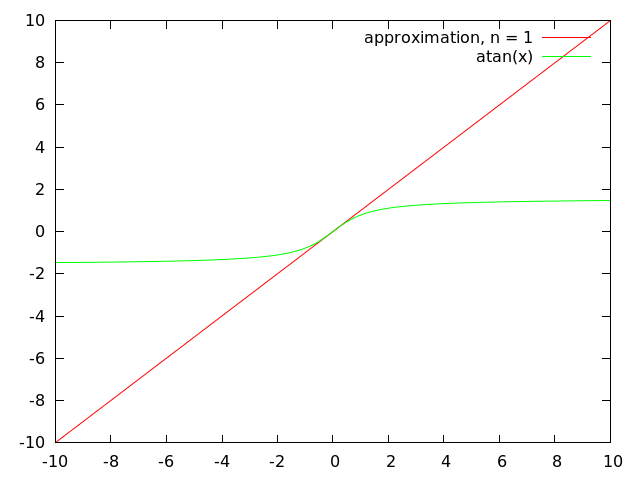
\includegraphics[scale=0.4,natwidth=640,natheight=480]{plot/atan1.png}\\
Wykres dla funkcji $\arctan$ przybliżonej pierwszym zbieżnikiem.

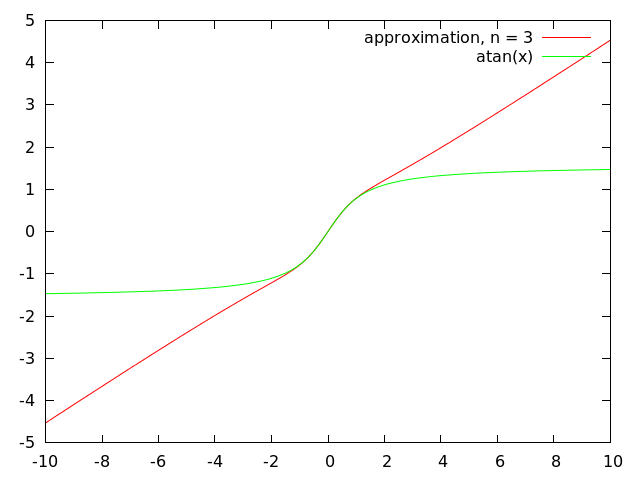
\includegraphics[scale=0.4,natwidth=640,natheight=480]{plot/atan3.png}\\
Wykres dla funkcji $\arctan$ przybliżonej trzecim zbieżnikiem.

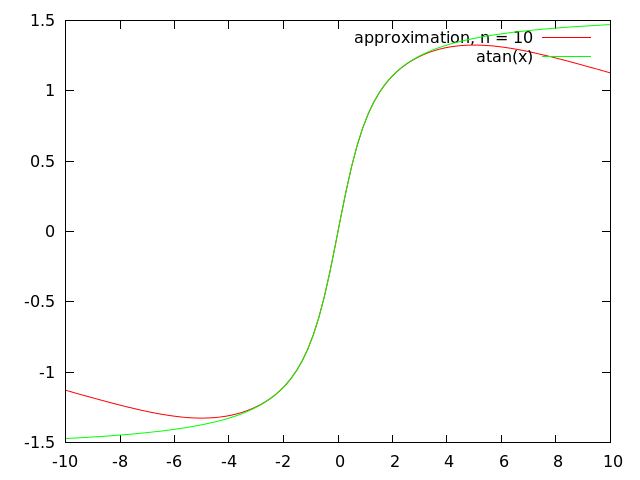
\includegraphics[scale=0.4,natwidth=640,natheight=480]{plot/atan10.png}\\
Wykres dla funkcji $\arctan$ przybliżonej dziesiątym zbieżnikiem.

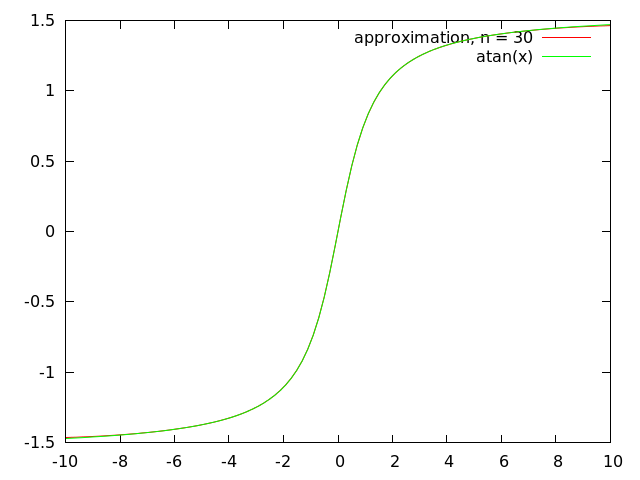
\includegraphics[scale=0.4,natwidth=640,natheight=480]{plot/atan30.png}\\
Wykres dla funkcji $\arctan$ przybliżonej trzydziestym zbieżnikiem.
\end{center}

Widać więc, że dla trzeciego zbieżnika otrzymano całkiem dobre przyblizenie funkcji $\arctan$ na przedziale $[-1, 1]$, dla szóstego na przedziale $[-2, 2]$, dla trzydziestego na przedziale $[-10, 10]$. Pozwala to sądzić, że $a$-ty zbieżnik daje dosyć dokładne przybliżenia wartości funkcji $\arctan$ na przedziale $[-\frac{a}{3}, \frac{a}{3}]$. To oznacza bardzo złą wiadomość dla metody ,,schodami w górę''. Ponieważ jest ona w stanie udźwignąć tylko ułamki co najwyżej dwudziestopiętrowe, przybliżanie funkcji na większych przedziałach jest w jej przypadku niemożliwe.

Poniżej zaprezentowano średnią wartość bezwzględną błędu (porównując do funkcji bibliotecznej) dla obydwu metod na przedziale $[-10, 10]$ w zależności od ilości iteracji (zbieżnika).

\begin{center}
\begin{tabular}{ r || r | r }
  \hline
  n & ,,w górę'' & ,,w dół''\\
  \hline \hline
  1 & 3.7595264911651611 & 3.7595264911651611 \\
  2 & 0.7099433541297913 & 0.7099433541297913 \\
  3 & 1.1721245050430298 & 1.1721243858337402 \\
  4 & 0.4252121150493622 & 0.4252121150493622 \\
  5 & 0.5263023972511292 & 0.5263024568557739 \\
  6 & 0.2582738399505615 & 0.2582737803459167 \\
  7 & 0.2708774805068970 & 0.2708774507045746 \\
  8 & 0.1578368544578552 & 0.1578368395566940 \\
  9 & 0.1495293229818344 & 0.1495293080806732 \\
  10 & 0.0968518778681755 & 0.0968518704175949 \\
  15 & 0.0306686945259571 & 0.0306686889380217 \\
  20 & 0.0089374929666519 & 0.0089374836534262 \\
  21 & 0.0071938033215702 & NaN \\
  22 & 0.0056154360063374 & NaN \\
  23 & 0.0045042322017252 & NaN \\
  24 & 0.0035408260300756 & NaN \\
  25 & 0.0028349994681776 & NaN \\
  30 & 0.0009046627092175 & NaN \\
\end{tabular}
\end{center}

\subsection{Przybliżanie wartości liczby $\pi$}
Do przybliżania wartości $\pi$ treść zadania sugeruje następujący ułamek łańcuchowy
\[
\frac{4}{\pi}
=
1 + \frac{1^2}{\displaystyle
  2 + \frac{3^2}{\displaystyle
    2 + \frac{5^2}{\displaystyle
      2 + \frac{7^2}{\displaystyle
        2 + \dots
      }
    }
  }
}
\]
Ułamek ten bardzo wolno zbiega do wartości $\frac{4}{\pi} \approx 1.27323954473516268615107$. W poniższej tabeli zaprezentowano wyniki dla kolejnych iteracji.

\begin{center}
\begin{tabular}{ r || r | r }
  \hline
  n & ,,w górę'' & ,,w dół''\\
  \hline \hline
  1 & 1.5000000000000000 & 1.5000000000000000 \\
  2 & 1.1538461446762085 & 1.1538461446762085 \\
  3 & 1.3815789222717285 & 1.3815789222717285 \\
  4 & 1.1977186203002930 & 1.1977186203002930 \\
  5 & 1.3440651893615723 & 1.3440651893615723 \\
  10 & 1.2375028133392334 & 1.2375028133392334 \\
  15 & 1.2990584373474121 & 1.2990581989288330 \\
  20 & 1.2542390823364258 & 1.2542388439178467 \\
  25 & 1.2890146970748901 & 1.2890143394470215 \\
  30 & 1.2603020668029785 & NaN \\
  50 & 1.2653428316116333 & NaN \\
  100 & 1.2692395448684692 & NaN \\
  1000 & 1.2728347778320312 & NaN \\
\end{tabular}
\end{center}

Inną opcją przybliżania wartości $\pi$ jest skorzystanie z funkcji $\arctan$, którą jak wiadomo z poprzedniego przykładu w łatwy sposób można przybliżyć z dość dobrą dokładnością już dla 30 iteracji. Wystarczy więc wykorzystać fakt, że $\arctan(1) = \frac{\pi}{4}$. Jeszcze inną możliwością jest skorzystanie z następującego ułamka (który to swoją drogą jest szczególnym przypadkiem innego wzoru na funkcję $\arctan$)
\[
\pi
=
3 + \frac{1^2}{\displaystyle
  6 + \frac{3^2}{\displaystyle
    6 + \frac{5^2}{\displaystyle
      6 + \dots
    }
  }
}
\]
Stosując ten ułamek można otrzymać wyniki dużo szybciej zbiegające do dokładnej wartości $\pi$. Niestety, tak jak poprzednio, od 26 iteracji metoda ,,schodami w dół'' zaczyna zwracać wartości NaN. Na poniższych wykresach widać jednak, że dla parzystych zbieżników ,,schodami w dół'' daje niewiele lepsze (ale i również mniej stabilne) wyniki niż ,,schodami w górę''.

\begin{center}
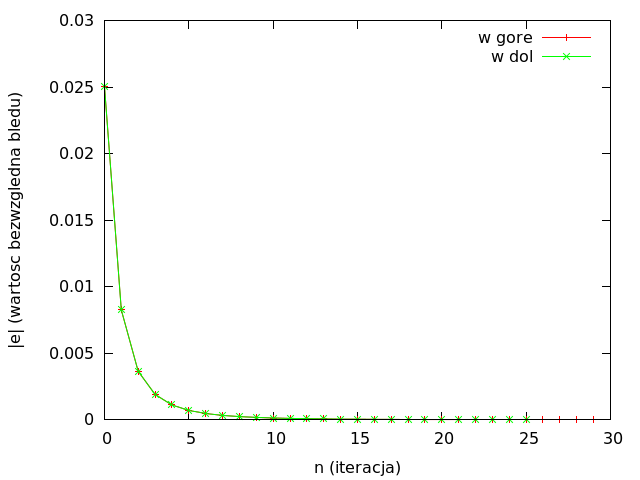
\includegraphics[scale=0.65,natwidth=640,natheight=480]{plot/pi30err.png}\\
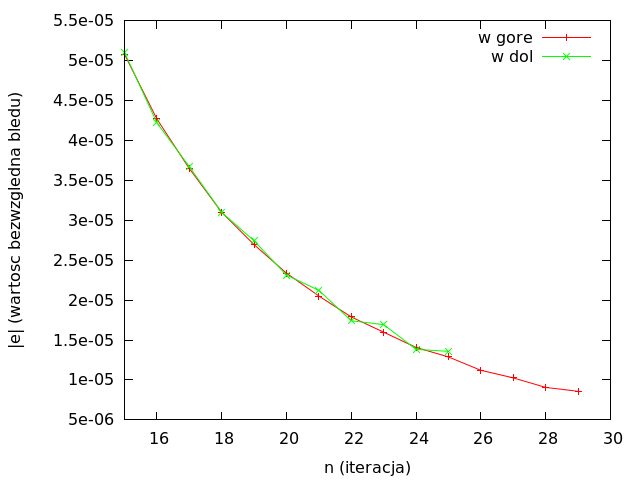
\includegraphics[scale=0.65,natwidth=640,natheight=480]{plot/pi30errzoom.png}\\
\end{center}

\subsection{Przybliżanie wartości liczby $e$}
Do przybliżania wartości stałej $e$ wykorzystywany będzie następujący ułamek łańcuchowy
\[
e
=
2 + \frac{2}{\displaystyle
  2 + \frac{3}{\displaystyle
    3 + \frac{4}{\displaystyle
      4 + \dots
    }
  }
}
\approx
2.718281828459045235
\]

Na podstawie poniższej tabeli można wyciągnąć mylny wniosek, że metoda ,,schodami w górę'' utyka w pewnym momencie przestając zwiększać swoją dokładność. Okazuje się jednak, że jest to najdokładniejsza wartość liczby $e$, która daje się reprezentować w arytmetyce pojedynczej precyzji. To oznacza, że najdokładnieszy możliwy wynik zostaje osiągnięty już po 8 iteracjach!

\begin{center}
\begin{tabular}{ r || r | r }
  \hline
  n & ,,w górę'' & ,,w dół''\\
  \hline \hline
  1 & 3.0000000000000000 & 3.0000000000000000 \\
  2 & 2.6666667461395264 & 2.6666667461395264 \\
  3 & 2.7272727489471436 & 2.7272727489471436 \\
  4 & 2.7169811725616455 & 2.7169811725616455 \\
  5 & 2.7184464931488037 & 2.7184464931488037 \\
  6 & 2.7182633876800537 & 2.7182633876800537 \\
  7 & 2.7182836532592773 & 2.7182836532592773 \\
  8 & 2.7182817459106445 & 2.7182817459106445 \\
  9 & 2.7182817459106445 & 2.7182817459106445 \\
  10 & 2.7182817459106445 & 2.7182817459106445 \\
  15 & 2.7182817459106445 & 2.7182819843292236 \\
  20 & 2.7182817459106445 & 2.7182822227478027 \\
  25 & 2.7182817459106445 & 2.7182815074920654 \\
  30 & 2.7182817459106445 & 2.7182812690734863 \\
  31 & 2.7182817459106445 & 2.7182812690734863 \\
  32 & 2.7182817459106445 & 2.7182812690734863 \\
  33 & 2.7182817459106445 & NaN \\
  100 & 2.7182817459106445 & NaN \\
  500 & 2.7182817459106445 & NaN \\
  1000 & 2.7182817459106445 & NaN \\
\end{tabular}
\end{center}

Wnioski dla metody ,,schodami w górę'' można wyciągnąć z poniższych wykresów. Widać, że algorytm przed osiągnięciem NaN w pewnych momentach dostaje najdokładniejszą wartość w pewnej iteracji po to, by w następnym kroku zacząć się od niej oddalać. Potwierdza to niestabilność metody ,,schodami w górę'' zaobserwowaną wcześniej również dla przybliżania liczby $\pi$. 

\begin{center}
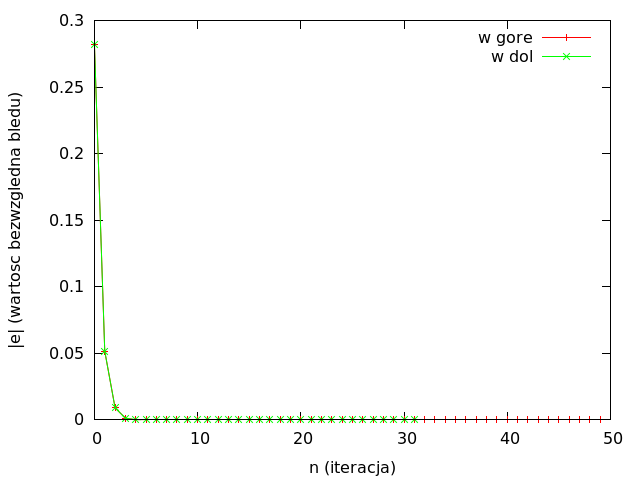
\includegraphics[scale=0.65,natwidth=640,natheight=480]{plot/e50err.png}\\
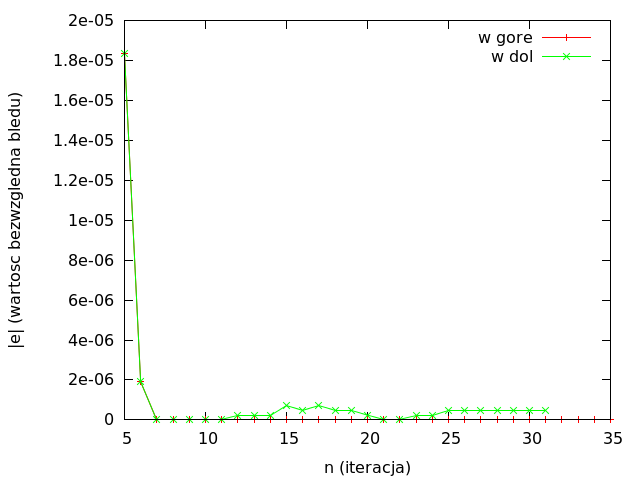
\includegraphics[scale=0.65,natwidth=640,natheight=480]{plot/e50errzoom.png}\\
\end{center}


\section{Wnioski}

Na podstawie powyższych przykładów można wyciągnąć wniosek, że najprostszy pomysł w tym przypadku okazuje się być tym najlepszym. Metoda ,,schodami w górę'' radzi sobie nie tylko z bardzo wysokimi ułamkami ale również okazuje się być dużo bardziej stabilna od swojej konkurentki.

Druga metoda może być jednak przydatna gdy zachodzi potrzeba wyznaczania ciągu zbieżników. Ma ona także cechy typowo ,,iteracyjne'' - mając wynik dla $n$-tego zbieżnika w razie potrzeby można doliczyć kolejne przybliżenia. Wspinając się ,,do góry'' nie da się wykorzystać wiedzy na temat $n$-tego zbieżnika do obliczenia $n+1$ i trzeba cały proces ewaluacji powtarzać od nowa dla większego ułamka. To spora wada, ponieważ znacząco komplikuje zadania wymagające obliczania wartości z określoną granicą błędu.

\begin{thebibliography}{99}
\bibitem{WikiCF} http://en.wikipedia.org/wiki/Continued fraction
\bibitem{AoSC} Numerical Recipes in Fortran: The Art of Scientific Computing
\bibitem{Cruyssen} P. Van der Cruyssen, A continued fraction algorithm, Numerische Mathematik 37 (1981)
\end{thebibliography}

\end{document}